% указываем класс документа
\documentclass[12pt,a4paper,openany]{extarticle}

% подключаем собственный стилевой файл 
\usepackage{mystyle}

% указываем язык (для автоматической вставки слов, типа "Глава", "Содержание", "Литература", "рис." и пр.
\selectlanguage{russian}

\begin{document}
\part*{Лабораторная работа №5б\\
Разработка системы управления для неполноприводного робота.\\ {\LARGE Часть~1.~Построение математической модели объекта управления.}}

\section{Методические рекомендации}
\hspace*{\parindent}Перед изучением материала пособия следует освоить содержание документа <<Лабораторная работа~№5а~\dots Часть~1~\dots>>. 

\section{Теоретические сведения}
\hspace*{\parindent}Данная версия 5-ой работы посвящена робототехническому устройству, обычно именуемому как <<Segway>>.
Его примерный вид можно видеть на рис.~\ref{main_segway_photo}.

\begin{figure}[h]
	\noindent\centering{ 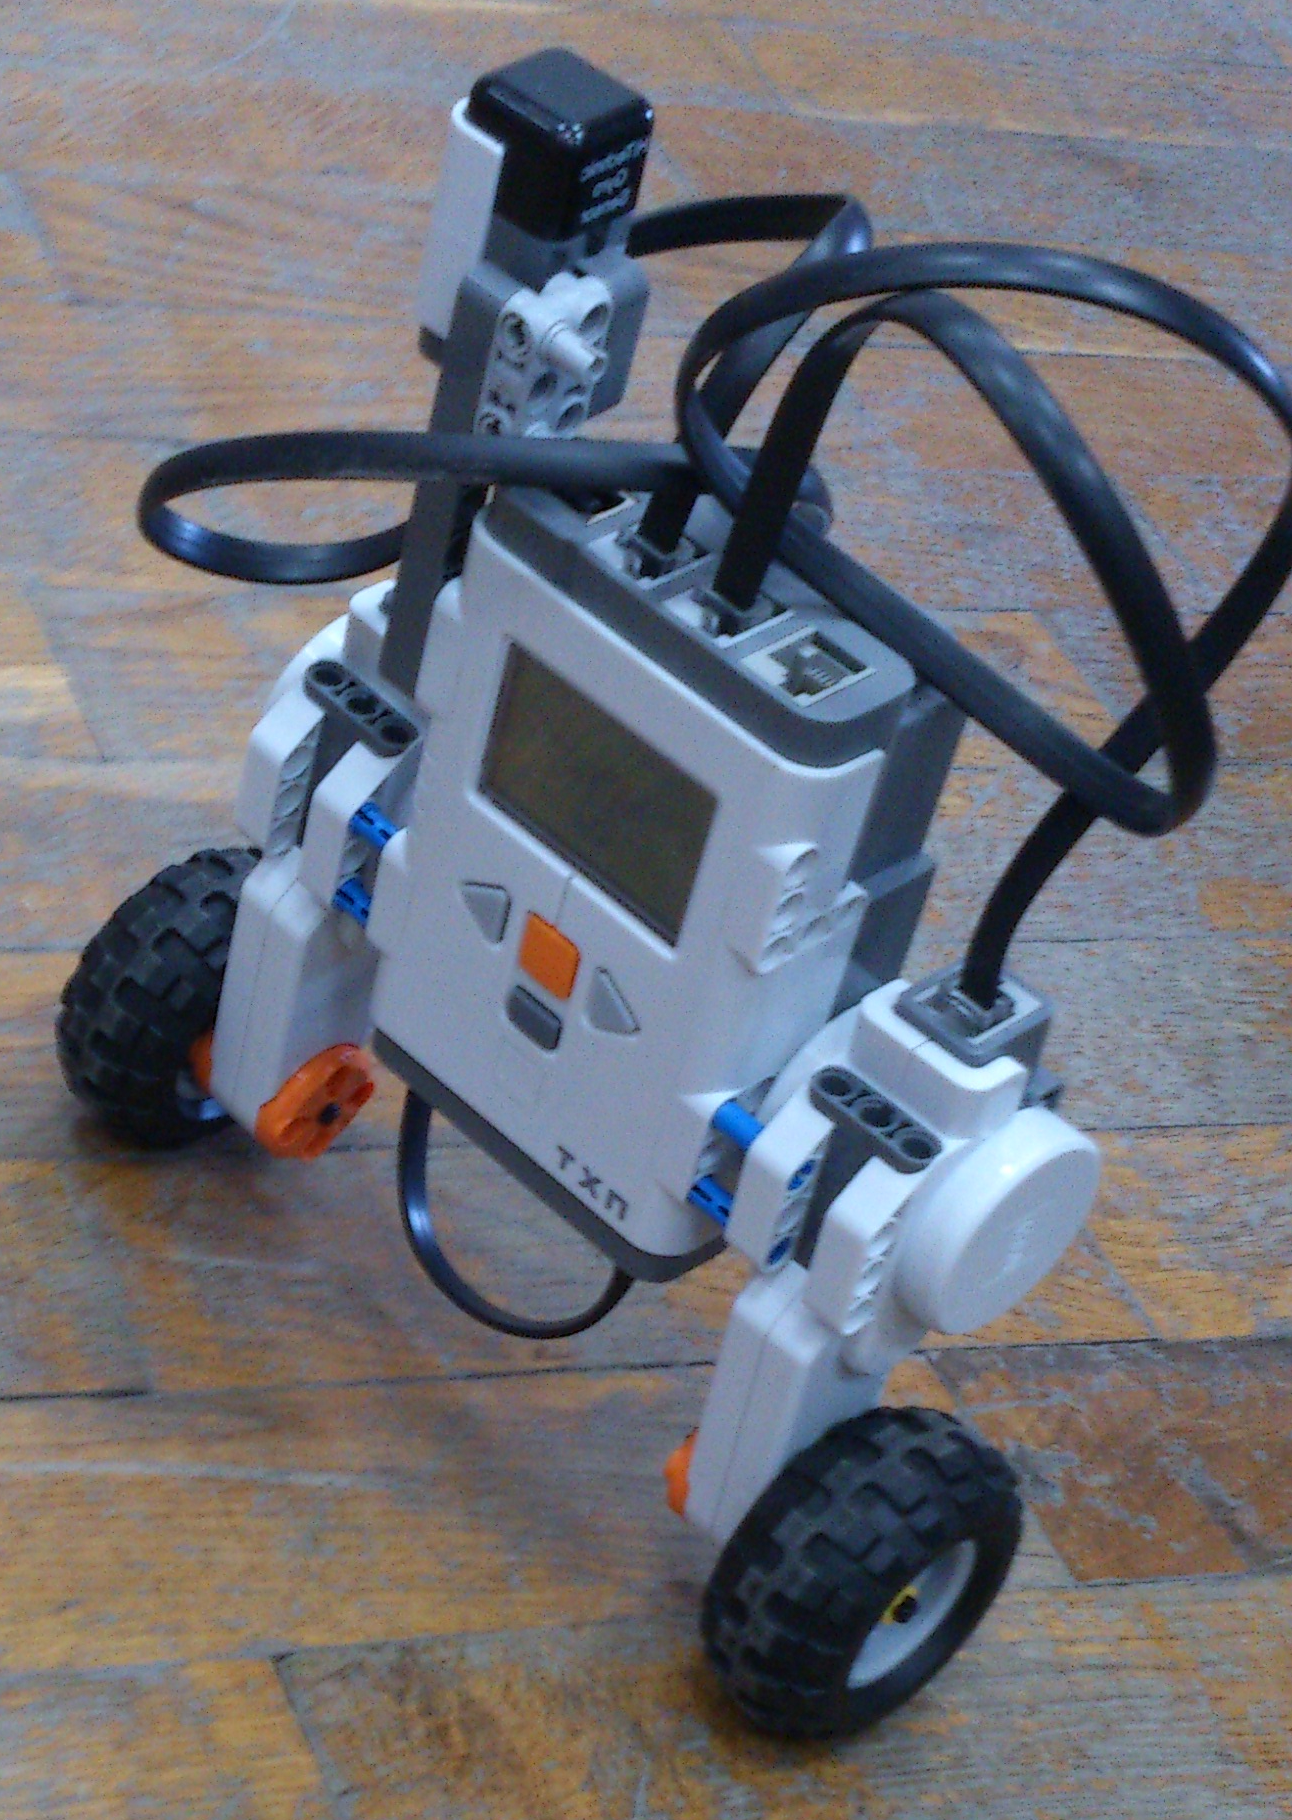
\includegraphics[scale=0.2]{main_segway_photo.png} }
	\caption{Примерный вид робота Segway.}
	\label{main_segway_photo}
\end{figure}

Segway представляет из себя одноосного колесного робота, который, перемещаясь в двух противоположных направлениях, способен удерживать свое <<тело>> в вертикальном положении.

\newpage
\paragraph*{Математическая модель}$\phantom{-}$\\
\hspace*{\parindent}Аналогично тому, как это было сделано в документе <<Лабораторная работа~№5а~\dots Часть~1~\dots>>, для Segway можно получить, что он имеет всего две степени свободы\lefteqn,\footnote{Опять предполагается, что его колеса не проскальзывают.} и положение в пространстве в любой момент времени каждого из составляющих его тел можно однозначно определить, используя всего две обобщенные координаты~--- угол поворота колес из начального положения ($\theta$) и угол отклонения робота от вертикали ($\psi$).   
Выражения, связывающие их с обычными декартовыми координатами центра масс <<тела>> робота ($x_\text{т},\ y_\text{т}$) и центра масс колес ($x_\text{к},\ y_\text{к}$) имеют вид (рис.~\ref{segway_in_decart}):
\begin{gather}
	x_\text{к} = x_\text{к}^{(0)} + r\theta, \label{xk}\\
	y_\text{к} = const,\\
	x_\text{т} = x_\text{к} + |CW|\sin\psi,\\
	y_\text{т} = y_\text{к} + |CW|\cos\psi \label{yt}
\end{gather} 
где $x_\text{к}^{(0)}$~--- значение коодинаты $x_\text{к}$ в начальный момент времени; $r$~--- радиус колеса; $|CW|$~--- длина отрезка $CW$, обозначим которую через $l$.

\begin{figure}[h]
	\noindent\centering{ 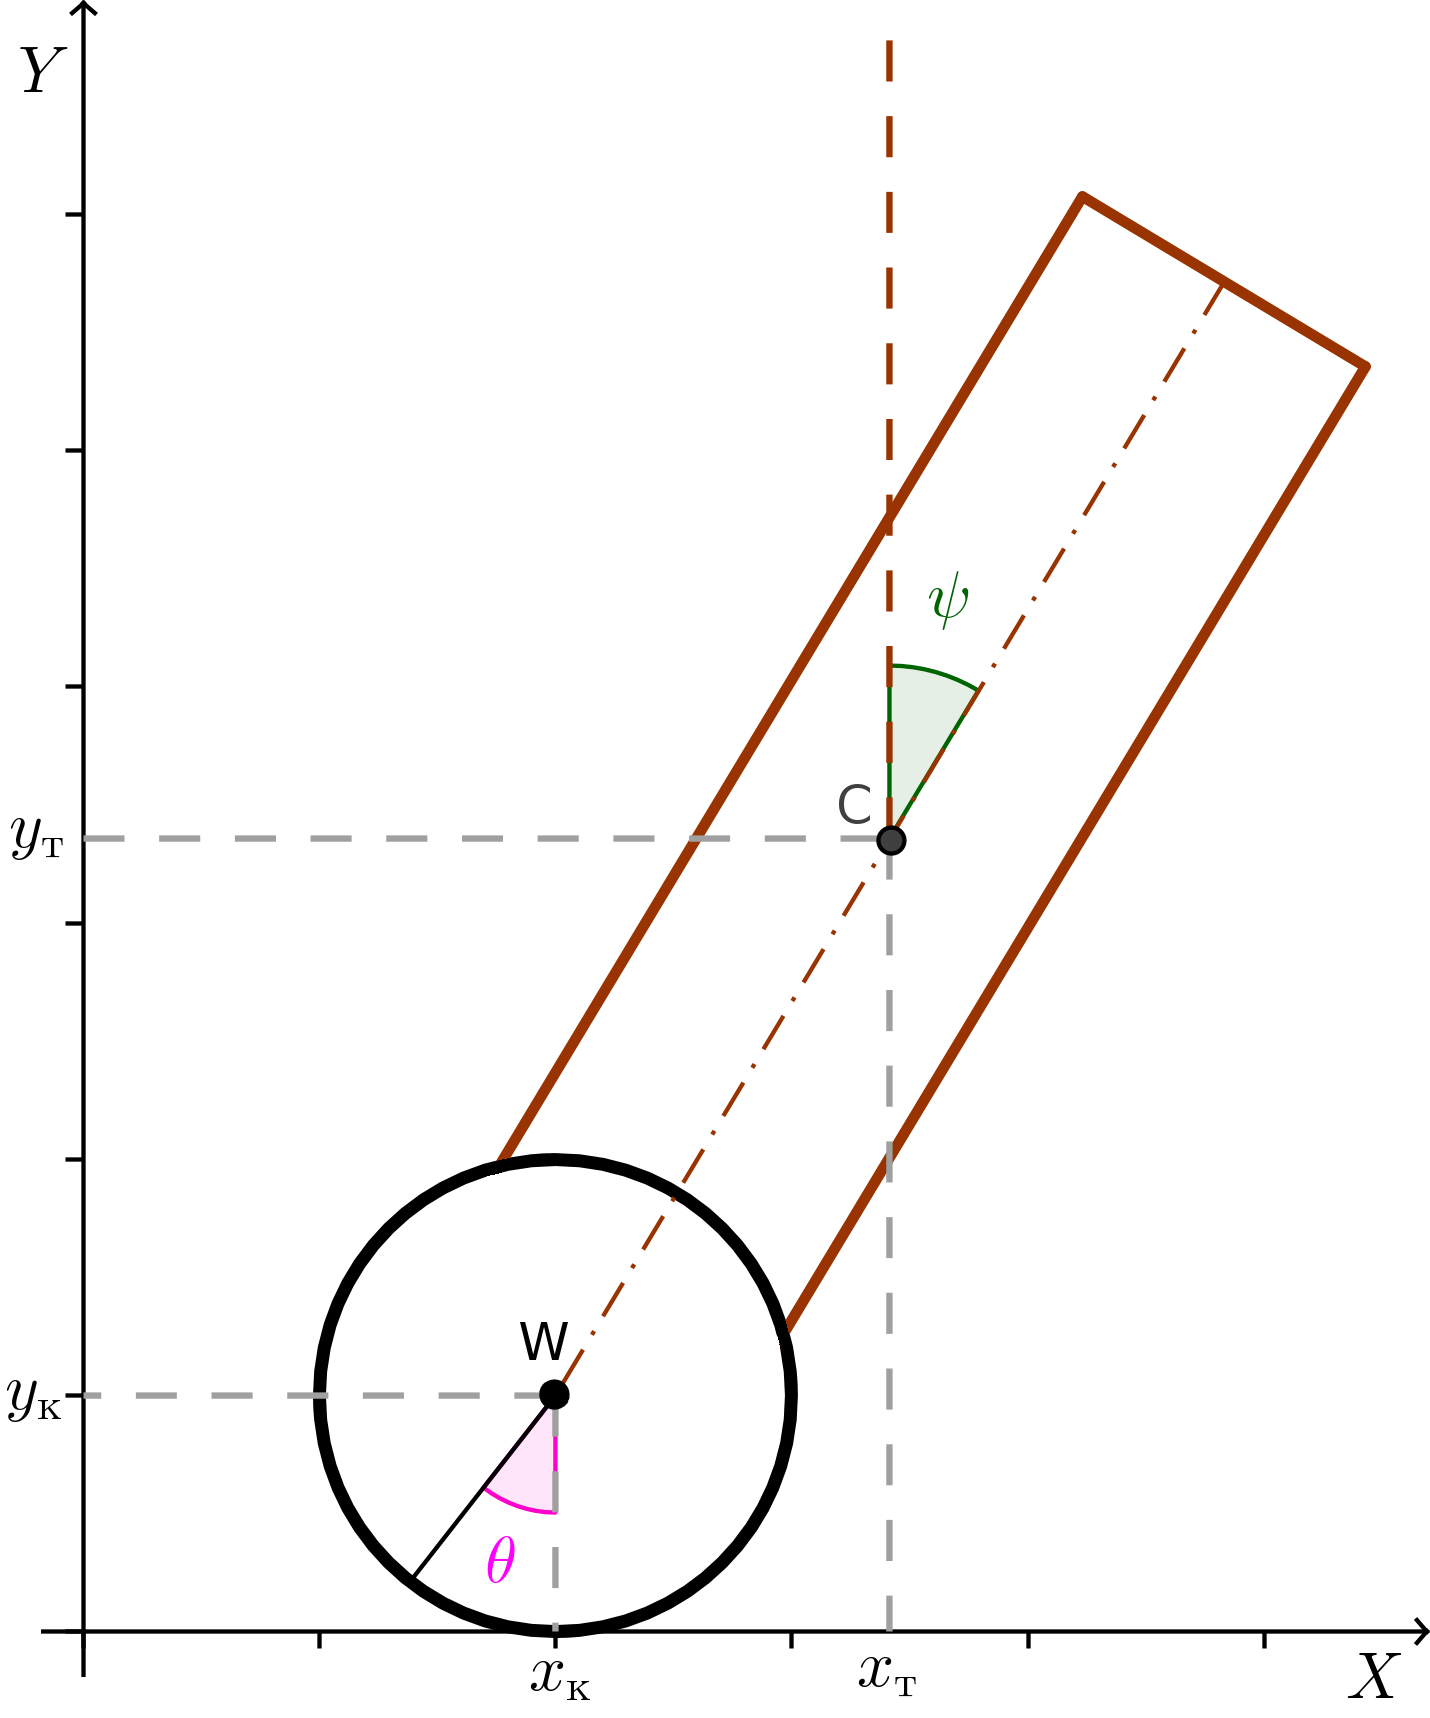
\includegraphics[scale=1.2]{segway_in_decart.png} }
	\caption{Робот в прямоугольной системе кординат.}
	\label{segway_in_decart}
\end{figure}

Законы Ньютона для колес и <<тела>> Segway с учетом действующих в системе сил (рис.~\ref{forces}\footnote{Двойки перед обозначениями момента $M$ опущены для экономии места на рисунке. На самом деле они нужны, поэтому считайте, что они подразумеваются.}) запишутся в виде:\\
для <<тела>>:
\begin{align}
	&m_\text{т}\ddot{x}_\text{т} = N_x, \label{mtax}  &&\text{(второй закон в проекции на ось $OX$)}\\	
	&m_\text{т}\ddot{y}_\text{т} = N_y - m_\text{т}g, \label{mtay}  &&\text{(второй закон в проекции на ось $OY$)}\\
	&J_\text{т}\ddot\psi  = N_yl\sin\psi - N_xl\cos\psi - 2M; \label{Jt}  &&\text{(уравнение моментов)}\\
\intertext{для колес:}
	&2m_\text{к}\ddot{x}_\text{к} = F_\text{тр} - N_x, \label{mkax}  &&\text{(второй закон в проекции на ось $OX$)}\\	
	&2J_\text{к}\ddot\theta = 2M - F_\text{тр}r; \label{Jk}  &&\text{(уравнение моментов)}
\end{align}
где $m_\text{т}$ и $m_\text{к}$~--- массы <<тела>> и одного колеса соответственно; $J_\text{т}$ и $J_\text{к}$~--- их моменты инерции относительно собственных центров масс; $N$~--- сила реакции, действующая между колесами и <<телом>> (индексами отмечены ее проекции на соответствующие оси); $M$~--- момент, с которым мотор раскручивает колеса (всего в конструкции их два, поэтому стоит  множитель, равный двум); $F_\text{тр}$~--- сила трения, действующая на колеса.
Несложно видеть, что последние два уравнения записаны сразу для пары колес, а не для каждого по отдельности.

\begin{figure}[h]
	\noindent\centering{ 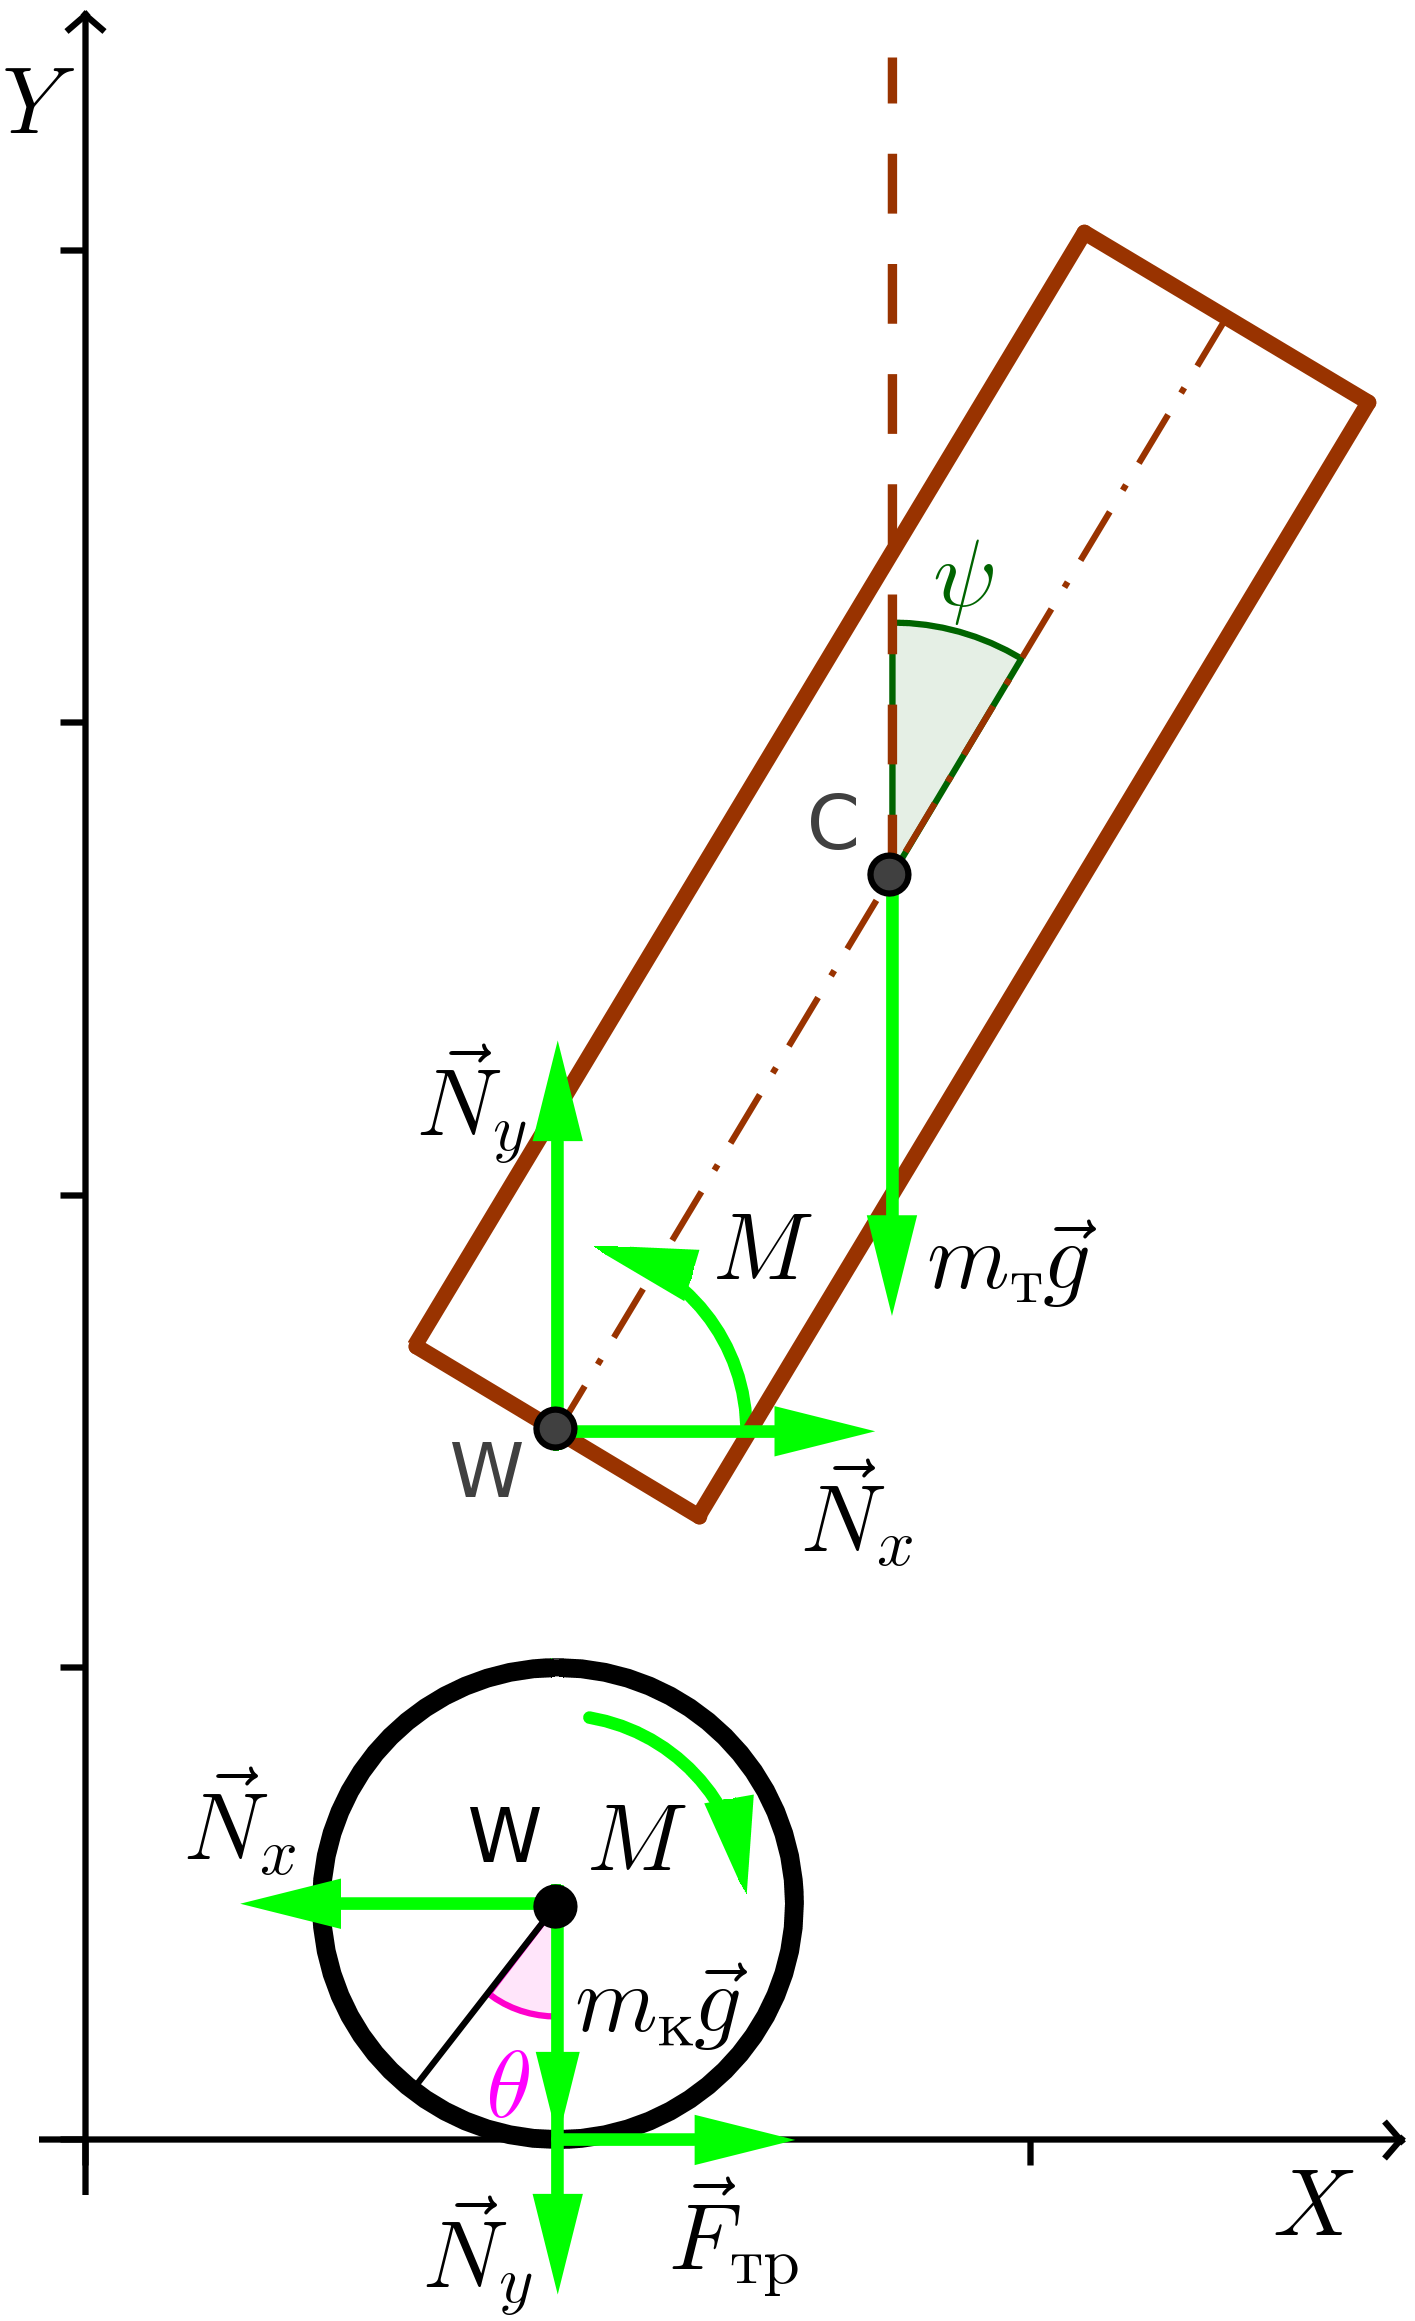
\includegraphics[scale=1]{forces.png} }
	\caption{Действующие в системе силы.}
	\label{forces}
\end{figure}

Важно отметить, что в случае с Segway на отклонение его <<тела>> от вертикали непосредственное влияние будет оказывать суммарный вращательный момент, создаваемый двигателями (см.~уравнение~\eqref{Jt}).
В~нашей ситуации это является следствием из третьего закона Ньютона.
Данная особенность представляет из себя главное отличие между текущей моделью обратного маятника и той, которая была рассмотрена в другой версии этой лабораторной работы.

Для того, чтобы убрать из полученных выражений неизвестные силы $F_\text{тр}$ и $N$, во-первых, выразим $N_x$ из~\eqref{mtax}, $N_y$ из~\eqref{mtay} и подставим результаты в уравнения~\eqref{Jt} и~\eqref{mkax}, а во-вторых, выразим $F_\text{тр}$ из~\eqref{mkax} и подставим ее в выражение~\eqref{Jk}.
В~итоге получим
\begin{equation}\label{system_witn_x&ys}
	\left\{
	\begin{aligned}
		\!&J_\text{т}\ddot\psi = \left(m_\text{т}g + m_\text{т}\ddot{y}_\text{т}\right)l\sin\psi - m_\text{т}\ddot{x}_\text{т}l\cos\psi 
			-2M\\
		\!&2J_\text{к}\ddot\theta = 2M - 2m_\text{к}\ddot{x}_\text{к}r - m_\text{т}\ddot{x}_\text{т}r\ldotp
	\end{aligned}
	\right.
\end{equation}

С~учетом того, что, согласно выражениям~\eqref{xk}~--~\eqref{yt}, справедливы следующие равенства:
\begin{gather}
	\ddot{x}_\text{к} = r\ddot\theta, \label{dxk}\\
	\ddot{y}_\text{к} = 0,\\
	\ddot{x}_\text{т} = r\ddot\theta + l\ddot\psi\cos\psi -l\dot\psi^2\sin\psi,\\
	\ddot{y}_\text{т} = -l\ddot\psi\sin\psi - l\dot\psi^2\cos\psi, \label{dyt}
\end{gather}
сделаем в системе~\eqref{system_witn_x&ys} соответствующие подстановки; в итоге будем иметь
\begin{equation}\label{system_witnout_x&ys}
	\left\{
	\begin{aligned}
		\!&J_\text{т}\ddot\psi = m_\text{т}gl\sin\psi - m_\text{т}l^2\ddot\psi - m_\text{т}lr\ddot\theta\cos\psi -2M\\
		\!&2J_\text{к}\ddot\theta = 2M - 2m_\text{к}r^2\ddot\theta - m_\text{т}r^2\ddot\theta - m_\text{т}lr\ddot\psi\cos\psi +
		 	m_\text{т}lr\dot{\psi}^2\sin\psi\ldotp
	\end{aligned}
	\right.
\end{equation}

Теперь достигнем этого же результата, используя уравнения Лагранжа.

Составим выражения для механических энергий входящих в Segway тел.
Получим\\
для <<тела>>:
\begin{align}
	&T_\text{п}^{(\text{т})} = \frac12m_\text{т}\left(\dot x_\text{т}^2 + \dot y_\text{т}^2\right)\!, \label{Tpt}  
		&&\text{(для поступательного движения центра масс)}\\	
	&T_\text{в}^{(\text{т})} = \frac12J_\text{т}\dot\psi^2\!\!, \label{Tvt}  &&\text{(для вращательного движения отн.~центра масс)}\\
	&U^{(\text{т})} = m_\text{т}gy_\text{т}; \label{Ut} &&\text{(потенциальная энергия)}\\
\intertext{для колес:}
	&T_\text{п}^{(\text{к})} = 2\cdot\frac12m_\text{к}\left(\dot x_\text{к}^2 + \dot y_\text{к}^2\right)\!, \label{Tpt}  
		&&\text{(для поступательного движения центра масс)}\\	
	&T_\text{в}^{(\text{к})} = 2\cdot\frac12J_\text{к}\dot\theta^2\!\!, \label{Tvt}  
		&&\text{(для вращательного движения отн.~центра масс)}\\
	&U^{(\text{к})} = 2m_\text{к}gy_\text{к}. \label{Ut} &&\text{(потенциальная энергия)}
\end{align}
Подставляя в эти выражения уравнения~\eqref{dxk}~--~\eqref{dyt}, окончательно получим:\\
для <<тела>>:
\begin{align}
	&T_\text{п}^{(\text{т})} = \frac12m_\text{т}\left(r^2\dot\theta^2 + 2lr\dot\psi\dot\theta\cos\psi + l^2\dot\psi^2\right)\!, \label{Tpt+} 
		&&\text{(для поступательного движения центра масс)}\\	
	&T_\text{в}^{(\text{т})} = \frac12J_\text{т}\dot\psi^2\!\!, \label{Tvt+}  &&\text{(для вращательного движения\dots)}\\
	&U^{(\text{т})} = C + m_\text{т}gl\cos\psi; \label{Ut+} &&\text{(потенциальная энергия)}\\
\intertext{для колес:}
	&T_\text{п}^{(\text{к})} = m_\text{к}r^2\dot\theta^2\!\!, \label{Tpt+}  &&\text{(для поступательного движения центра масс)}\\	
	&T_\text{в}^{(\text{к})} = J_\text{к}\dot\theta^2\!\!, \label{Tvt+}  &&\text{(для вращательного движения\dots)}\\
	&U^{(\text{к})} = const, \label{Ut+} &&\text{(потенциальная энергия)}
\end{align}
где $C$~--- некоторая константа.

Функция Лагранжа, которая в этом случае вычисляется по формуле
\begin{equation}
	L = 	T_\text{п}^{(\text{т})} + T_\text{в}^{(\text{т})} + T_\text{п}^{(\text{к})} + T_\text{в}^{(\text{к})} 
		- U^{(\text{т})} - U^{(\text{к})}\!,
\end{equation}
распишется как
\begin{equation}
	L =  \frac12m_\text{т}r^2\dot\theta^2 + m_\text{т}lr\dot\psi\dot\theta\cos\psi + \frac12m_\text{т}l^2\dot\psi^2 +
	\frac12J_\text{т}\dot\psi^2 + m_\text{к}r^2\dot\theta^2 + J_\text{к}\dot\theta^2 - C - m_\text{т}gl\cos\psi - U^{(\text{к})}\!\ldotp
\end{equation}

Для составления уравнений Лагранжа посмотрим, какие силы и моменты сил\footnote{Напоминаем, что силы реакции и потенциальные силы рассматривать не нужно.} будут совершать работы при малых положительных увеличениях обобщенных координат.
Если дать координате $\psi$ приращение $\delta\psi$ (рис.~\ref{forces}), то работу, равную $-2M\delta\psi$, совершит только суммарный момент, создаваемый сервоприводами, следовательно в правую часть соответствующего уравнения следует записать $-2M\delta\psi/\delta\psi = -2M$.
Если же положительное увеличение $\delta\theta$ дать координате $\theta$, то опять работу, равную $2M\delta\theta$, совершат только моменты $M$. 
Отсюда аналогичным образом имеем, что в правую часть второго уравнения  следует записать $2M\delta\theta/\delta\theta = 2M$.

С учетом выше сказанного получим следующие уравнения Лагранжа:
\begin{equation}
	\left\{  
	\begin{aligned}
		\!&\frac{d}{dt}\frac{\partial L}{\partial\dot{\psi}} - \frac{\partial L}{\partial\psi} = -2M\\
		\!&\frac{d}{dt}\frac{\partial L}{\partial\dot{\theta}} - \frac{\partial L}{\partial \theta} = 2M\ldotp
	\end{aligned}   
	\right.
\end{equation}
Выполнив необходимые операции дифференцирования, будем иметь
\begin{gather}
	\frac{\partial L}{\partial\dot{\psi}} = m_\text{т}lr\dot\theta\cos\psi + m_\text{т}l^2\dot\psi + J_\text{т}\dot\psi,\\
	\frac{d}{dt}\frac{\partial L}{\partial\dot{\psi}} = m_\text{т}lr\ddot\theta\cos\psi - m_\text{т}lr\dot\psi\dot\theta\sin\psi + 
		m_\text{т}l^2\ddot\psi + J_\text{т}\ddot\psi,\\
	\frac{\partial L}{\partial\psi} = -m_\text{т}lr\dot\psi\dot\theta\sin\psi + m_\text{т}gl\sin\psi, \\
	\frac{\partial L}{\partial\dot{\theta}} = m_\text{т}r^2\dot\theta + m_\text{т}lr\dot\psi\cos\psi + 2m_\text{к}r^2\dot\theta +
		2J_\text{к}\dot\theta,\\
	\frac{d}{dt}\frac{\partial L}{\partial\dot{\theta}} = m_\text{т}r^2\ddot\theta + m_\text{т}lr\ddot\psi\cos\psi -
		m_\text{т}lr\dot\psi^2\sin\psi + 2m_\text{к}r^2\ddot\theta + 2J_\text{к}\ddot\theta,\\
	\frac{\partial L}{\partial \theta} = 0\ldotp	
\end{gather}
Подставив их в уравнения Лагранжа, окончательно получим
\begin{equation}\label{from_lagr's_eqs}
	\left\{
	\begin{aligned}
		\!&m_\text{т}lr\ddot\theta\cos\psi + m_\text{т}l^2\ddot\psi + J_\text{т}\ddot\psi - m_\text{т}gl\sin\psi = -2M\\
		\!&m_\text{т}r^2\ddot\theta + m_\text{т}lr\ddot\psi\cos\psi - m_\text{т}lr\dot\psi^2\sin\psi + 2m_\text{к}r^2\ddot\theta + 
			2J_\text{к}\ddot\theta = 2M\ldotp
	\end{aligned}
	\right.
\end{equation}
Несложно убедится, что эти уравнения совпадают с теми, которые представлены в системе~\eqref{system_witnout_x&ys}.

Заменив в полученных выражениях функцию $M$ по формуле:
\begin{equation}
	M = \frac{k_m}{R}U - \frac{k_mk_e}{R}\dot\theta - J\ddot\theta,
\end{equation}
будем иметь
\begin{equation}\label{from_lagr's_eqs_without_M}
	\left\{
	\begin{aligned}
		\!&m_\text{т}lr\ddot\theta\cos\psi + m_\text{т}l^2\ddot\psi + J_\text{т}\ddot\psi - m_\text{т}gl\sin\psi - 2J\ddot\theta -
			\frac{2k_mk_e}{R}\dot\theta  = -\frac{2k_m}{R}U\\
		\!&m_\text{т}r^2\ddot\theta + 2m_\text{к}r^2\ddot\theta + 2J_\text{к}\ddot\theta + 2J\ddot\theta + m_\text{т}lr\ddot\psi\cos\psi -
			m_\text{т}lr\dot\psi^2\sin\psi  + \frac{2k_mk_e}{R}\dot\theta= \frac{2k_m}{R}U,
	\end{aligned}
	\right.
\end{equation}
а линеаризовав эти уравнения, окончательно получим
\begin{equation}\label{final_eqs}
	\left\{
	\begin{aligned}
		\!&m_\text{т}lr\ddot\theta + m_\text{т}l^2\ddot\psi + J_\text{т}\ddot\psi - m_\text{т}gl\psi - 2J\ddot\theta - 
			\frac{2k_mk_e}{R}\dot\theta  = -\frac{2k_m}{R}U\\
		\!&m_\text{т}r^2\ddot\theta + 2m_\text{к}r^2\ddot\theta + 2J_\text{к}\ddot\theta + 2J\ddot\theta + m_\text{т}lr\ddot\psi +
		\frac{2k_mk_e}{R}\dot\theta= \frac{2k_m}{R}U,
	\end{aligned}
	\right.
\end{equation}

Последние две пары уравнений представляют собой искомую математическую модель робота соответственно в обычной и линеаризованной формах.
В заключение перепишем полученные выражения в матричном виде.

Введем следующие обозначения:
\begin{gather}
	q = 
	\begin{bmatrix}
		\theta\\
		\psi
	\end{bmatrix}\!\!, 
	\\
	u = U.
\end{gather}
С~учетом их запишем систему~\eqref{final_eqs} в виде
\begin{equation}
	E\ddot{q} + F\dot{q} + Gq = Hu
\end{equation}
где
\begin{gather}
	E = 
	\begin{bmatrix}
		m_\text{т}lr - 2J & m_\text{т}l^2 +  J_\text{т}\\
		m_\text{т}r^2 + 2m_\text{к}r^2 + 2J_\text{к} + 2J & m_\text{т}lr
	\end{bmatrix}\!\!,\;
	F = 
	\begin{bmatrix}
		-\cfrac{2k_mk_e}{R} & \phantom{!}0\phantom{!}\\
		\cfrac{2k_mk_e}{R} & 0
	\end{bmatrix}\!\!,\;
	G =
	\begin{bmatrix}
		0 & -m_\text{т}gl\\
		\phantom{!}0\phantom{!} & 0	
	\end{bmatrix}\!\!,\notag\\
	H = 
	\begin{bmatrix}
		-\cfrac{2k_m}{R}\\
		\cfrac{2k_m}{R}
	\end{bmatrix}\!\!,\qquad
	\dot{q} =
	\begin{bmatrix}
		\dot{\theta}\\
		\dot{\psi}
	\end{bmatrix}\!\!,\qquad
	\ddot{q} =
	\begin{bmatrix}
		\ddot{\theta}\\
		\ddot{\psi}
	\end{bmatrix}\!\!\ldotp			 
\end{gather}
Выразим из полученного уравнения матрицу $\ddot{q}$, умножив его на матрицу $E^{-1}$ слева и перебросив некоторые слагаемые  в правую часть:
\begin{equation}
	\ddot{q}=-E^{-1}F\dot{q} - E^{-1}Gq + E^{-1}Hu,
\end{equation}
где
\begin{gather}
	E^{-1} = 
	\begin{bmatrix}
		\cfrac{m_\text{т}lr}{\varkappa_1} & -\cfrac{m_\text{т}l^2 + J_\text{т}}{\varkappa_1}\\
		-\cfrac{m_\text{т}r^2 + 2m_\text{к}r^2 + 2J_\text{к} + 2J}{\varkappa_1} & \cfrac{m_\text{т}lr - 2J}{\varkappa_1}
	\end{bmatrix}\!\!,\;\\
	E^{-1}F = 
	\begin{bmatrix}
		-\cfrac{2k_mk_e\left(m_\text{т}lr + m_\text{т}l^2 + J_\text{т}\right)}{R\varkappa_1} & \phantom{!}0\phantom{!}\\
		\cfrac{2k_mk_e\left(m_\text{т}lr + m_\text{т}r^2 + 2m_\text{к}r^2 + 2J_\text{к}\right)}{R\varkappa_1} & 0
	\end{bmatrix}\!\!,\;		
\end{gather}
\begin{gather}
	E^{-1}G = 
	\begin{bmatrix}
		\phantom{!}0\phantom{!} & -\cfrac{m_\text{т}^2gl^2r}{\varkappa_1}\\
		0 & \cfrac{m_\text{т}gl\left(m_\text{т}r^2 + 2m_\text{к}r^2 + 2J_\text{к} + 2J\right)}{\varkappa_1}
	\end{bmatrix}\!\!,\;\\
	E^{-1}H = 
	\begin{bmatrix}
		-\cfrac{2k_m\left(m_\text{т}lr + m_\text{т}l^2 + J_\text{т}\right)}{R\varkappa_1} \\
		\cfrac{2k_m\left(m_\text{т}lr + m_\text{т}r^2 + 2m_\text{к}r^2 + 2J_\text{к}\right)}{R\varkappa_1} 
	\end{bmatrix}\!\!,
\end{gather} 
где, в свою очередь,
\begin{equation}
	\varkappa_1 = m_\text{т}lr (m_\text{т}lr - 2J) - \left(m_\text{т}l^2 + J_\text{т}\right)\left(m_\text{т}r^2 + 2m_\text{к}r^2 + 2J_\text{к} + 2J\right) 	
		\!\ldotp
\end{equation}

Приводя получившееся выражение обратно в форму системы, будем иметь
\begin{equation}
	\left\{  
	\begin{aligned}
		\!&\ddot\theta = \cfrac{2k_mk_e\left(m_\text{т}lr + m_\text{т}l^2 + J_\text{т}\right)}{R\varkappa_1}\,\dot\theta +
		\cfrac{m_\text{т}^2gl^2r}{\varkappa_1}\,\psi 
		-\cfrac{2k_m\left(m_\text{т}lr + m_\text{т}l^2 + J_\text{т}\right)}{R\varkappa_1} \,U\\
		%
		\!&\begin{split}
			\ddot\psi = -\cfrac{2k_mk_e\left(m_\text{т}lr + m_\text{т}r^2 + 2m_\text{к}r^2 + 2J_\text{к}\right)}
			{R\varkappa_1}\,\dot\theta &-
			\cfrac{m_\text{т}gl\left(m_\text{т}r^2 + 2m_\text{к}r^2 + 2J_\text{к} + 2J\right)}{\varkappa_1}\,\psi\ +\\
		&+ \cfrac{2k_m\left(m_\text{т}lr + m_\text{т}r^2 + 2m_\text{к}r^2 + 2J_\text{к}\right)}{R\varkappa_1}\,U.
		\end{split}
	\end{aligned}   
	\right.
\end{equation}
Добавим в полученную систему дополнительное уравнение:
\begin{equation}\label{math_model}
	\left\{  
	\begin{aligned}
		\!& \dot{\psi} = \dot{\psi} \\
		\!&\ddot\theta = \cfrac{2k_mk_e\left(m_\text{т}lr + m_\text{т}l^2 + J_\text{т}\right)}{R\varkappa_1}\,\dot\theta +
		\cfrac{m_\text{т}^2gl^2r}{\varkappa_1}\,\psi 
		-\cfrac{2k_m\left(m_\text{т}lr + m_\text{т}l^2 + J_\text{т}\right)}{R\varkappa_1} \,U\\
		%
		\!&\begin{split}
			\ddot\psi = -\cfrac{2k_mk_e\left(m_\text{т}lr + m_\text{т}r^2 + 2m_\text{к}r^2 + 2J_\text{к}\right)}
			{R\varkappa_1}\,\dot\theta &
			-\cfrac{m_\text{т}gl\left(m_\text{т}r^2 + 2m_\text{к}r^2 + 2J_\text{к} + 2J\right)}{\varkappa_1}\,\psi\ +\\
		&+ \cfrac{2k_m\left(m_\text{т}lr + m_\text{т}r^2 + 2m_\text{к}r^2 + 2J_\text{к}\right)}{R\varkappa_1}\,U.
		\end{split}
	\end{aligned}   
	\right.
\end{equation}
Введя обозначение
\begin{equation}
	x =
	\begin{bmatrix}
		\psi \\
		\dot{\theta} \\
		\dot{\psi}
	\end{bmatrix}\!\!,
\end{equation}
перепишем математическую модель робота в виде
\begin{equation}
	\dot x = Ax + Bu,
\end{equation}
где 
\begin{equation}
	A =
	\begin{bmatrix}
		0 & 0 & \phantom{!}1\phantom{!} \\
		\cfrac{m_\text{т}^2gl^2r}{\varkappa_1} & \cfrac{2k_mk_e\left(m_\text{т}lr + m_\text{т}l^2 + J_\text{т}\right)}
			{R\varkappa_1} & 0\\
		-\cfrac{m_\text{т}gl\left(m_\text{т}r^2 + 2m_\text{к}r^2 + 2J_\text{к} + 2J\right)}{\varkappa_1} &
			-\cfrac{2k_mk_e\left(m_\text{т}lr + m_\text{т}r^2 + 2m_\text{к}r^2 + 2J_\text{к}\right)}{R\varkappa_1} & 0
	\end{bmatrix}\!\!,
\end{equation}
\begin{equation}	
	B = 
	\begin{bmatrix}
		0 \\
		-\cfrac{2k_m\left(m_\text{т}lr + m_\text{т}l^2 + J_\text{т}\right)}{R\varkappa_1} \\
		\cfrac{2k_m\left(m_\text{т}lr + m_\text{т}r^2 + 2m_\text{к}r^2 + 2J_\text{к}\right)}{R\varkappa_1}
	\end{bmatrix}\!\!\ldotp
\end{equation}


\paragraph*{Схема моделирования}$\phantom{-}$\\
\hspace*{\parindent}Как видно из его математической модели, схема моделирования работы Segway полностью совпадает с той, которая была построена для обратного маятника на тележке (рис.~\ref{struct_sheme}).

\begin{figure}[h]
	\noindent\centering{ 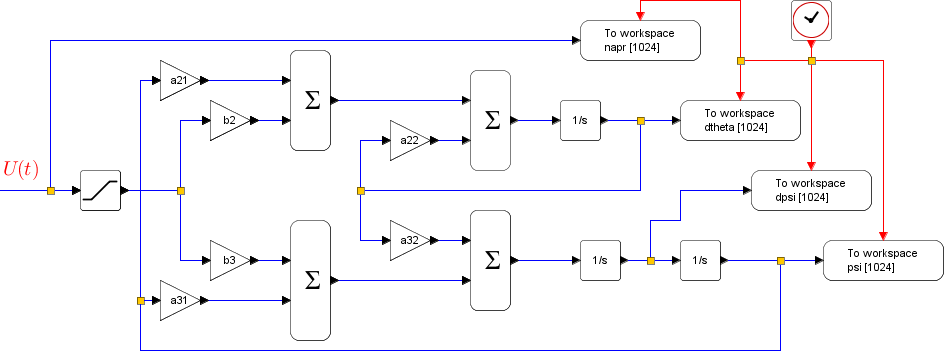
\includegraphics[scale=0.7]{struct_sheme.png} }
	\caption{Cхема моделирования работы устройства.}
	\label{struct_sheme}
\end{figure}

Единственное отличие заключается в том, что будет иной расшифровка входящих в схему переменных:
\begin{align}
	a22 &= \cfrac{2k_mk_e\left(m_\text{т}lr + m_\text{т}l^2 + J_\text{т}\right)}{R\varkappa_1} &
	a32 &= -\cfrac{2k_mk_e\left(m_\text{т}lr + m_\text{т}r^2 + 2m_\text{к}r^2 + 2J_\text{к}\right)}{R\varkappa_1}\notag \\
	a21 &= \cfrac{m_\text{т}^2gl^2r}{\varkappa_1} & 
	a31 &= -\cfrac{m_\text{т}gl\left(m_\text{т}r^2 + 2m_\text{к}r^2 + 2J_\text{к} + 2J\right)}{\varkappa_1} \\
	b2 &= -\cfrac{2k_m\left(m_\text{т}lr + m_\text{т}l^2 + J_\text{т}\right)}{R\varkappa_1} & 
	b3 &= \cfrac{2k_m\left(m_\text{т}lr + m_\text{т}r^2 + 2m_\text{к}r^2 + 2J_\text{к}\right)}{R\varkappa_1} \notag
\end{align}

\end{document}